% !TeX spellcheck = en_US
\documentclass[12pt, twoside]{article}

\usepackage[a4paper, top=2.5cm, bottom=2.5cm, left=3cm, right=2cm]{geometry}
\usepackage{ctex}
% \linespread{2.0}
\usepackage{times}
\usepackage{indentfirst}
\usepackage{multicol}
\setlength{\columnsep}{1cm}
\usepackage{wrapfig}
\usepackage{amsmath, amssymb, mathtools}
\usepackage{graphicx}
\usepackage{subfig}
\renewcommand{\thesubfigure}{Figure \arabic{subfigure}}
\captionsetup[subfigure]{labelformat=simple, labelsep=colon}
\graphicspath{{./images/}}
\usepackage[backend=biber]{biblatex}
\addbibresource{References.bib}
\usepackage{float}

\title{\textbf{An Overview on Supervised Learning in ML}}
\author{From: 快要变成猪了QwQ}
\date{}

\begin{document}	
\maketitle

%ABSTRACT
\noindent\textbf{Abstract: }\textit{Machine Learning} (ML) has seamlessly integrated into various aspects of daily life, spanning applications like spam filters, fraud detection, and personal advertising. Despite the growing familiarity with the term, a considerable number of individuals remain unfamiliar with its precise meaning, application, and the pivotal role of ML algorithms and datasets in the realm of data science. This article seeks to demystify ML by focusing on a specific branch, \textit{Supervised Learning} (SL). The article begins with an exploration of \textit{Regression} and \textit{Classification}, two key branches within SL. Initiating with the foundational 2-D \textit{Linear Regression Model}, the article progresses to elucidate concepts such as \textit{Features, Cost Function, and Gradient Descent,} subsequently extending the Linear Regression Model to higher dimensions through \textit{Multiple Features} and \textit{Vectorization}. The discourse then delves into practical Gradient Descent techniques, encompassing \textit{Feature Scaling, Convergence Checking, Learning Rate, Feature Engineering,} and \textit{Polynomial Regression}. Shifting to Classification within SL, the introduction of the \textit{Sigmoid Function}, new \textit{Error Function} and \textit{Decision boundary} is discussed. The article navigates through the awkward scenarios of \textit{Underfitting} and \textit{Overfitting}, facilitating readers in establishing intuitive insights into \textit{Bias and Variance} by visualizing the model. To strike a balance between Bias and Variance, the discussion veers towards \textit{Regularization}, a common \textit{optimization} practice among ML practitioners.The article concludes by addressing the limitations of ML and presenting a future perspective, motivating readers to explore advanced AI algorithms.
\vspace{20pt}

%KEYWORDS
\noindent\textbf{Keywords: }Machine Learning, Supervised Learning, Regression, Classification.
\vspace{20pt}

%THE MAINBODY
\begin{multicols*}{2}
	
\section{Introduction}
In the ever-expanding landscape of Machine Learning (ML), the fusion of Supervised Learning (SL) and Neural Networks stands as a cornerstone, driving unprecedented advancements and transforming diverse sectors. As ML permeates into every aspect of contemporary life, from spam filters and fraud detection to personalized advertising, understanding the fundamental concepts of Supervised Learning and Neural Networks becomes paramount.

Supervised Learning, a foundational paradigm within ML, operates on the principle of learning from labeled datasets. This approach involves training models to make predictions or decisions based on input data paired with corresponding output labels. The significance of supervised learning lies in its ability to generalize patterns from existing data, enabling accurate predictions on new, unseen data. This paper provides a comprehensive overview, unraveling the intricacies of Supervised Learning and its symbiotic relationship with Neural Networks.

Neural Networks, inspired by the complexity of the human brain, have emerged as powerful tools within the realm of Supervised Learning. These interconnected networks of nodes, or neurons, exhibit the capacity to capture intricate patterns and relation-ships in data. The structure of neural networks, encompassing layers and activation functions, forms the basis for their ability to process information in a way that mirrors human cognition.

As we navigate through the fol-lowing sections, we will delve into diverse details of training an ML model. The training process of neural networks, a pivotal aspect of super-vised learning, involves techniques such as gradient descent, where the model adjusts its parameters to minimize the difference between predicted and actual outcomes. Challenges such as overfitting and underfitting, common in supervised learning scenarios, necessitate the exploration of regularization methods to optimize model performance.

This paper not only aims to elucidate the foundational concepts of Supervised Learning but also endeavors to provide insights into their applications, challenges, and future trends. As we embark on this exploration, we will uncover the transformative potential of these ML paradigms and their role in shaping the future of artificial intelligence.
	
\section{Supervised Learning}
	\subsection{Definition}
	The learner receives a set of labeled examples as training data and makes predictions for all unseen points. This is the most common scenario associated with classification, regression, and ranking problems. The spam detection problem is an instance of supervised learning.\cite{enwiki:1188072476}\cite{mohri2018foundations}
		
	\subsection{Linear Regression}
		\subsubsection{Single Feature Linear Regression}
		Given a data set $\{x_i,y_i\}_{i=1}^{m}$, Linear Regression assumes that the correlation between feature $x_i$ and label $y_i$ is linear , i.e.,
		$$ \hat{y}=wx+e \triangleq f_{\mathbf{w},e}(x) $$
		and attempts to find a 'best' line to fit the data. To define the word 'best', \textit{Error} and \textit{Cost Function} are introduced.\cite{Altman2015PointsOS}
		
			\paragraph{Error}
			Error $e_i$ is defined as the deviation of $ y_i $ from the predicted value $f(x_i)$,
			$$ e_i = y_i - f(x_i). $$
			
			\paragraph{Cost Function}
			For Linear Regression, we apply the \textit{Squared Error} Cost Function
			$$J(w,e)=\frac{1}{2m}\sum_{i=1}^{m}e_i^2=\frac{1}{2m}\sum_{i=1}^{m}(y_i - f(x_i))^2$$
			to specify how well does the line $\hat{y}=wx+e $ fit the data set.
		
		Our ambiguous goal of finding a 'best' line to fit the data now converts into finding parameters $w$ and $e$ that minimizes the Cost Function.
		
		Intuitively, statisticians would have taken the partial derivatives of $J(w,e)$ and solve the two equations
		$$
		\begin{cases}
			\frac{dJ(w,e)}{dw}=0 \\
			\frac{dJ(w,e)}{de}=0
		\end{cases}.
		$$
		However, it is more sophisticated and less generalized to solve a system of partial derivatives than applying  Gradient Descent.
		
			\paragraph{Gradient Descent}
			Gradient Descent is an algorithm that finds a local minimum of a given function $f$.
			
			Gradient Descent is based on the observation that the function $f$ decreases fastest if one goes a tiny step from its current position $a$ in the direction of the negative gradient of $f$ at that point, $-\nabla f(a)$.\cite{enwiki:1187716577} In our example $J(\theta_1,\theta_2)$,
			$$ \nabla J(a)=\frac{\partial J}{\partial\theta_1}(a)+\frac{\partial J}{\partial\theta_2}(a) $$
			
			A Learning Rate $\alpha$ is selected to indicate how long a tiny step is. Therefore the big iterative formula of Gradient Descent comes like
			
			\begin{align*}
				&\text{Repeat until convergence \{}\\
					&\qquad\theta_1\coloneq\theta_1-\frac{\partial J}{\partial\theta_1}(\theta_1)\\
					&\qquad\theta_2\coloneq\theta_2-\frac{\partial J}{\partial\theta_2}(\theta_2)\\
				&\text{\}}
			\end{align*}
			
			\begin{figure}[H]
				\centering
				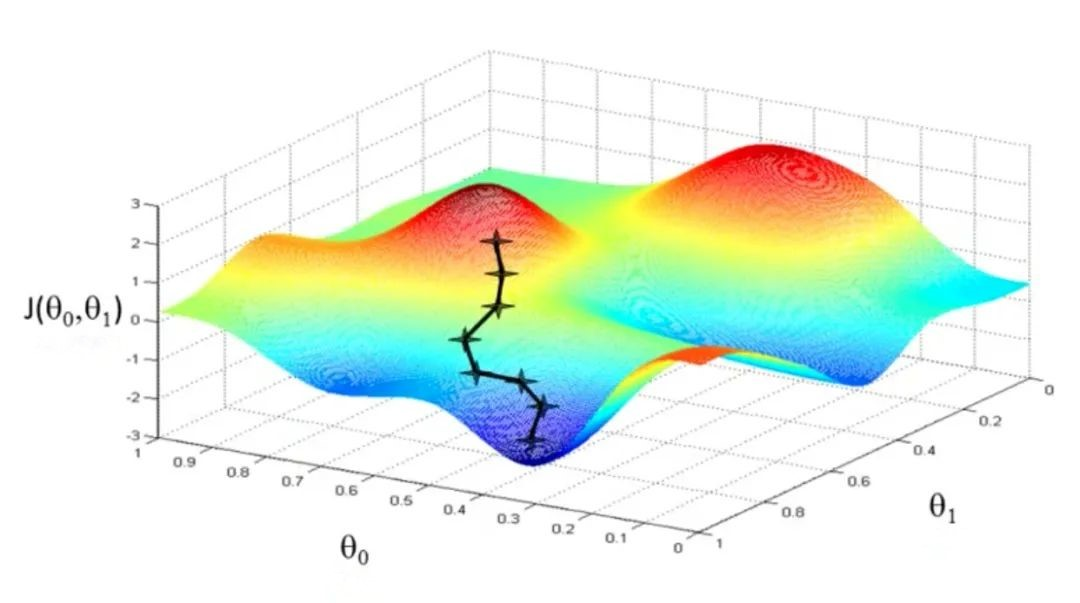
\includegraphics[width=\columnwidth]{gradient-descent-local-global-minimum}
				\caption{Plot of $J(\theta_1,\theta_2)$}
				\label{fig:GDplot1}
			\end{figure}
			
			From Figure \ref{fig:GDplot1} we discover that after several steps being taken, we are brought to one of the local minima of $J(\theta_1,\theta_2)$.
			
		Now let's veer back to the Squared Error Cost Function $J(w,e)$ and delve into one of its important properties, \textit{Convexity}.
		
		According to the definition of $ J(w,e)$, We deduce that
		\begin{align*}
			J(w,e) &= \frac{1}{2m}\sum_{i=1}^{m}(y_i - f(x_i))^2\\
			&= \frac{1}{2m}\sum_{i=1}^{m}(y_i - (wx_i+e))^2\\
			&= \frac{1}{2m}\sum_{i=1}^{m}
			\begin{aligned}[t]
				(&x_i^2w^2 + e^2 + 2x_iwe \\
				&- 2x_iy_iw -2y_ie + y_i^2)
			\end{aligned}
		\end{align*}
		which is saying that $J(w,e)$ is a quadratic function with respect to either $w$ or $e$. Therefore the Squared Error Cost Function is \textit{convex} and has only one global minimum, which implies that through Gradient Descent we can always minimize the Cost Function.
		\begin{figure}[H]
			\centering
			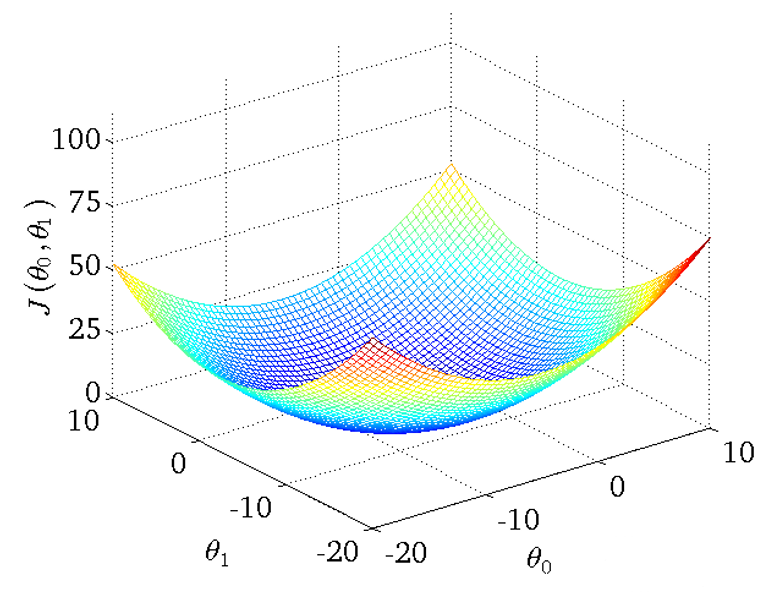
\includegraphics[width=\columnwidth]{convex-function}
			\caption{Plot of a convex function}
			\label{fig:Convex}
		\end{figure}
		
		Calculating the partial derivatives of $J(w,e)$:
		$$
		\begin{dcases}
			\frac{\partial J(w,e)}{\partial w}=\frac{1}{m}\sum_{i=1}^{m}(f(x_i)-y_i)w \\
			\frac{\partial J(w,e)}{\partial e}=\frac{1}{m}\sum_{i=1}^{m}(f(x_i)-y_i)
		\end{dcases}
		$$
		we obtain the iterative loop to minimize our Squared Error Cost Function $J(w,e)$,
		\begin{align*}
			&\text{Repeat until convergence \{}\\
				&\qquad w\coloneq w-\alpha\frac{\partial J(w,e)}{\partial w} \\
				&\qquad e\coloneq e-\alpha\frac{\partial J(w,e)}{\partial e} \\
			&\text{\}}
		\end{align*}
		
		\subsubsection{Multi-Features Linear Regression}
		It's barely impossible that mere one dimension of feature suffices the hunger of our model learning the pattern of data. We want out model to be capable of seeking correlations and making inferences using multiple features, that's where \textit{Vectorization} comes into play.
		
		We are now given a data set $\{x_i^{(1)},x_i^{(2)},\cdots,x_i^{(n)},y_i\}_{i=1}^{m}$ and want to find the 'best' line to fit the data. Therefore, we assume our model to be
		\begin{align*}
			\hat{y} &= w_1x^{(1)}+\cdots+w_nx^{(n)}+e \\
					&= \mathbf{w}^T\mathbf{x}+e\triangleq f_{\mathbf{w},e}(\mathbf{x})
		\end{align*}
		where $\mathbf{w}$ is a column vector comprised of parameters $w_1,\cdots,w_n$ and $\mathbf{x}$ is also a column vector comprised of input features $x_1,\cdots,x_n$.
		
		Similarly, the updating loop still applies.
		\begin{align*}
			&\text{Repeat until convergence \{}\\
				&\qquad w_i\coloneq w_i-\alpha\frac{\partial J(\mathbf{w},e)}{\partial w_i} \\
				&\qquad\qquad\qquad\text{for }i=1,2,\cdots,n \\
				&\qquad e\coloneq e-\alpha\frac{\partial J(w,e)}{\partial e} \\
			&\text{\}}
		\end{align*}
		
		\subsubsection{Gradient Descent In Practice}
			\paragraph{Feature Scaling}
			Feature Scaling is a method used to normalize the range of independent variables or features of data. In data processing, it is also known as data normalization and is generally performed during the data preprocessing step.\cite{enwiki:1177060479}
			
			The reason why we use this technique is that Gradient Descent converges way more faster with Feature Scaling than without it.\cite{ioffe2015batch}
			\begin{figure}[H]
				\centering
				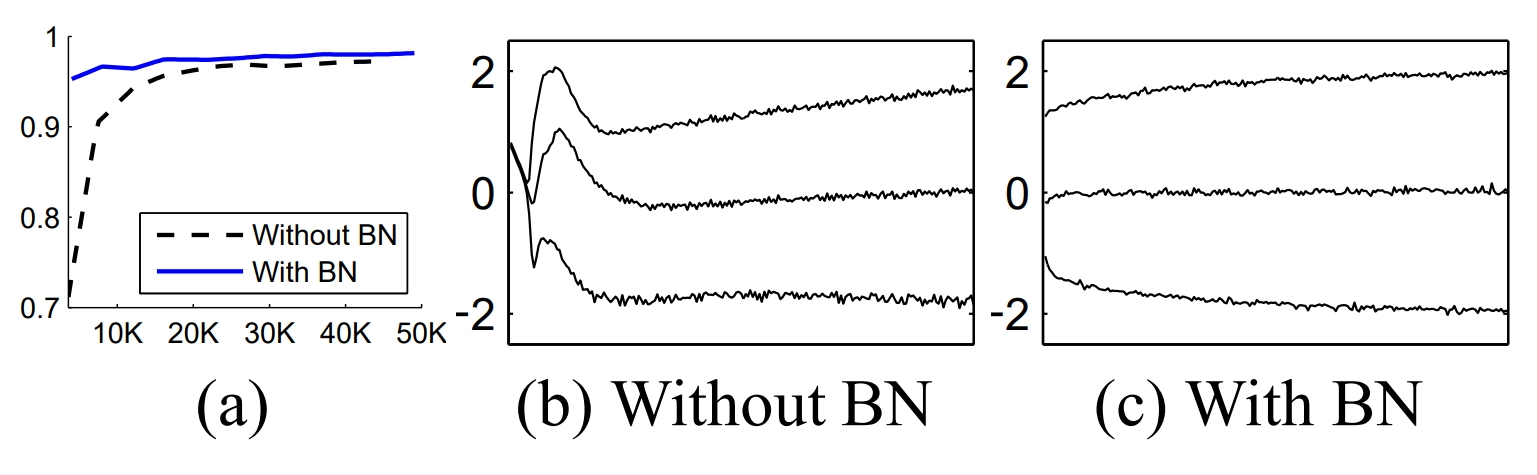
\includegraphics[width=\columnwidth]{BN-contrast}
				\caption{(a) The test accuracy of the MNIST network trained with and without Batch Normalization, vs. the number of training steps. Batch Normalization helps the network train faster and achieve higher accuracy. (b,c) The evolution of input distributions to a typical sigmoid, over the course of training, shown as {15, 50, 85}th percentiles. Batch Normalization makes the distribution more stable and reduces the internal co-variate shift.\cite{ioffe2015batch}}
				\label{fig:BN-contrast}
			\end{figure}
			
			Below are some typical types of Feature Scaling methods that ML practitioners apply to boost the performance of their model.
			\begin{itemize}
				\item \textbf{Rescaling} Also known as min-max scaling or min-max normalization, rescaling is the simplest method and consists in rescaling the range of features to scale the range in $[0,1]$ or $[-1,1]$. Selecting the target range depends on the nature of the data. The general formula for a min-max of $[0,1]$ is given as:
				$$ x'=\frac{x-\min(x)}{\max(x)-\min(x)} $$
				where $x$ is the original value, $x'$ is the normalized value. To rescale a range between an arbitrary interval $[a,b]$, the formula becomes:
				$$ x'=a+\frac{(x-\min(x))(b-a)}{\max{x}-\min{x}} $$
				
				\item \textbf{Mean Normalization}
				$$ x'=\frac{x-\bar{x}}{\max(x)-\min(x)} $$
				where $x$ is the original value, $ x'$ is the normalized value and $\bar{x}\triangleq\text{average}(x)$ is the mean of that feature vector.
				
				\item \textbf{Z-score Normalization} In machine learning, we can handle various types of data, e.g. audio signals and pixel values for image data, and this data can include multiple dimensions. Feature standardization makes the values of each feature in the data have zero-mean (when subtracting the mean in the numerator) and unit-variance. This method is widely used for normalization in many machine learning algorithms (e.g., support vector machines, logistic regression, and artificial neural networks). The general method of calculation is to determine the distribution mean and standard deviation for each feature. Next we subtract the mean from each feature. Then we divide the values (mean is already subtracted) of each feature by its standard deviation,
				$$ x'=\frac{x-\bar{x}}{\sigma} $$
				where $x$ is the original feature vector, $\bar{x}\triangleq\text{average}(x)$ is the mean of that feature vector and $\sigma$ is its standard deviation.
			\end{itemize}
			
			\paragraph{Learning Curve} Learning curves describe a system’s performance on a task as a function over some resource to solve that task. There can be a certain budget of that resource, limiting the amount of resources that can be spent. In the simplest case, the budget can be quantified by the number of examples the learner has observed before performing the task or number of iterations or time the learner spends in an environment. The performance is a measure that captures how well a task is solved (e.g., error rate or the value of cost function). Learning curves are an important source of information for making decisions on the following matters in machine learning\cite{mohr2022learning}:
			\begin{itemize}
				\item \textbf{Data Acquisition} The acquisition of how many more labels is (maybe economically) reasonable?
				
				\item \textbf{Early Stopping (of training a model)} If we are committed to some specific learner (a learning algorithm and its hyperparameters), we might want to minimize the training time or avoid overfitting.
				
				\item \textbf{Early Discarding (in model selection)} If we want to select from various models, we want to stop the evaluation of a candidate when we are sure that it is not competitive to the best-known solution.
			\end{itemize}
			
			Many techniques have been proposed to address either of these problems. This is typically done by modeling (or extrapolating) the learning curves and acting upon predictions from that model. These learning curve models vary in the type of queries they are able to answer and this article introduces the \textit{Iteration Learning Curve} that helps ML practitioners to determine whether or not a model is convergent:
			\begin{figure}[H]
				\centering
				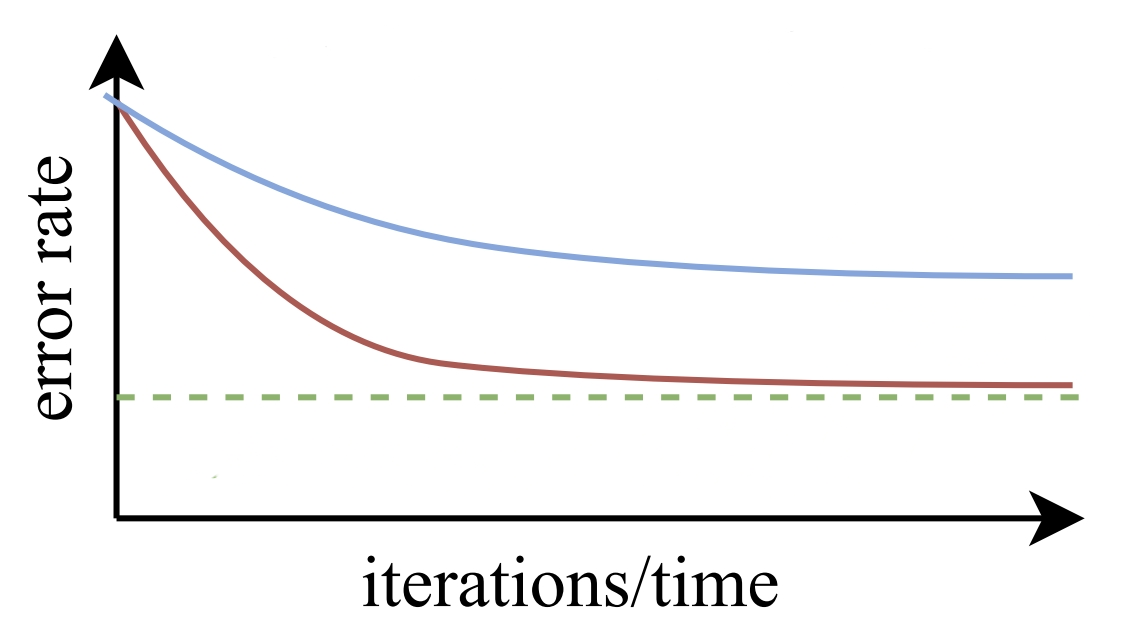
\includegraphics[width=\columnwidth]{learning-curve}
				\caption{Typical iteration learning curve\cite{mohr2022learning}}
				\label{fig:learning-curve}
			\end{figure}
			\noindent where the x-axis is number of iterations and the y-axis is value of $J(\mathbf{w},e)$
			
			Whenever iteration learning curve plateaus, or more specifically when $J(\mathbf{w},e)$ decreases by less than $\epsilon$ (a really small number like $10^{-3}$) in one iteration then it declares convergence.
			
			\paragraph{Feature Engineering} Suppose we are given features $x_1,x_2$ which represent frontage and depth of a house respectively
			\begin{figure}[H]
				\centering
				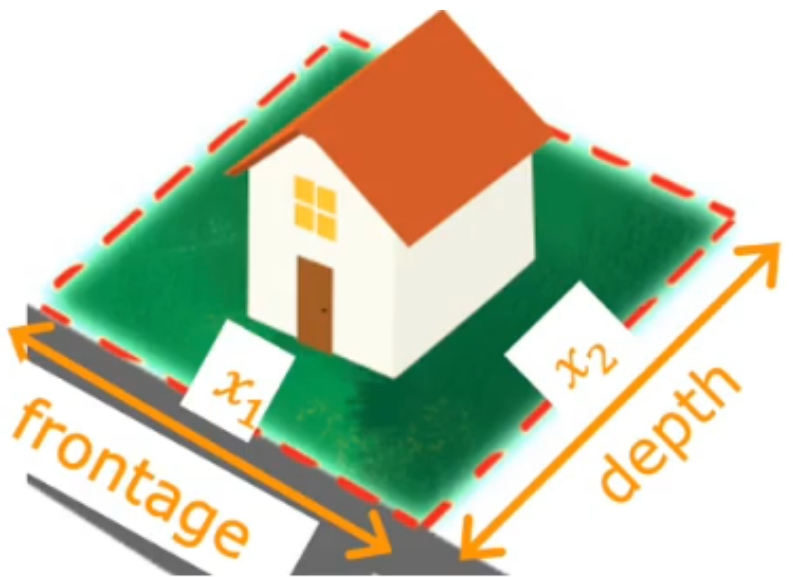
\includegraphics[width=\columnwidth]{feature-engineering}
				\caption{House price prediction}
			\end{figure}
			\noindent and we want to apply a linear regression model to predict the house price. Intuitively, we would assume that the area of house was more relevant than either frontage or depth of the house. Therefore a new feature $x_3=x_1x_2$ is manually engineered and the model becomes:
			$$ f_{\mathbf{w},e}(x)=w_1x_1+w_2x_2+w_3x_3+e $$
			
			This technique also applies to other scenarios where new features are designed using intuition and by transforming or combining original features.
			
			\paragraph{Polynomial Regression}
			The goal of regression analysis is to model the expected value of a dependent variable $y$ in terms of the value of an independent variable (or vector of independent variables) $x$. In simple linear regression, the relationship between $y$ and $x$ is linear. However in many settings, such a linear relationship may no longer holds.\cite{STIGLER1974431} For the example presented in Figure \ref{poly-eg}, a Polynomial Regression model
			$$ \hat{y}=w_1x+w_2x^2+w_3x^3+e $$
			is deployed and it fits the data better than simple linear regression.
			\begin{figure}[H]
				\centering
				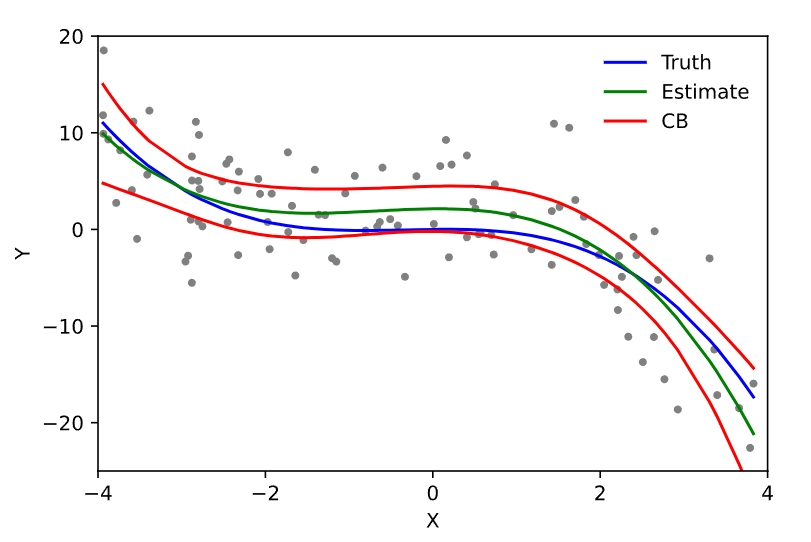
\includegraphics[width=\columnwidth]{Polyreg_scheffe}
				\caption{A cubic polynomial regression fit to a simulated data set.\cite{enwiki:1175712788}}
				\label{poly-eg}
			\end{figure}
			In general, we can model the expected value of $y$ as an $n$-th degree polynomial, yielding the general polynomial regression model
			\begin{align*}
				\hat{y} &= w_1x+w_2x^2+\cdots+w_mx^m+e\\
						&= \mathbf{w}^T\mathbf{x}+e\triangleq f_{\mathbf{w},e}(\mathbf{x})
			\end{align*}
			where $\mathbf{w}$ is a column vector consists of $w_1,w_2,\cdots,w_m$ and $\mathbf{x}$ is a column vector consists of $x,x^2,\cdots,x^m$.
			
	\subsection{Logistic Regression}
		\subsubsection{Limitation of Linear Regression}
		Linear regression has its limitations when it comes to classification problems. Like the data set in Figure \ref{fig:logis-eg},
		\begin{figure}[H]
			\centering
			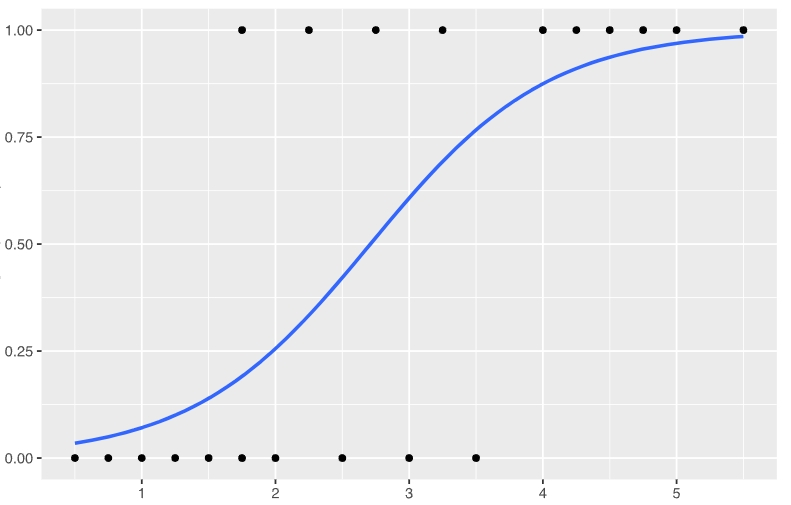
\includegraphics[width=\columnwidth]{logis-eg}
			\caption{Example graph of a logistic regression curve fitted to data.\cite{enwiki:1188449633}}
			\label{fig:logis-eg}
		\end{figure}
		\noindent it would be extremely counter-intuitive if we were to fit a line to it. Therefore we introduce \textit{Logistic Regression} to tackle this problem.
		
		\subsubsection{Sigmoid Function}
		Also known as \textit{Logistics Function}, sigmoid function is of the form:
		$$ g(z)=\frac{1}{1+e^{-z}} $$ 
		a graph of the sigmoid function on the interval $(-6,6)$ is shown in Figure \ref{fig:sigmoid}.
		\begin{figure}[H]
			\centering
			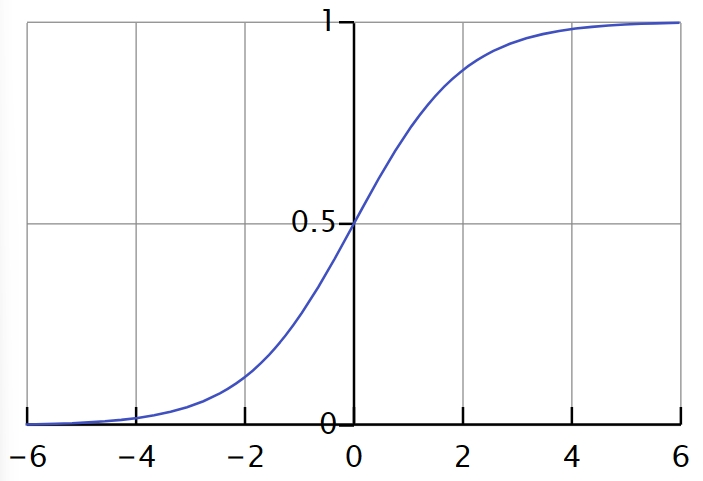
\includegraphics[width=\columnwidth]{sigmoid}
			\caption{Sigmoid Function.\cite{enwiki:1188449633}}
			\label{fig:sigmoid}
		\end{figure}
		\noindent Using certain degree of analogy, we let
		$$ z=\mathbf{w}^T\mathbf{x}+e $$
		and inserting that linear function $z$ into $g(z)$ we obtain
		$$
		f_{\mathbf{w},e}(\mathbf{x})=
		g(\underbrace{\mathbf{w}^T\mathbf{x}+e}_z)=
		\frac{1}{1+e^{\mathbf{w}^T\mathbf{x}+e}}
		$$
		\noindent a graph of logistic regression applied on tumor detection is show in Figure \ref{fig:logis-eg2} to help establish intuition on linear function $z$ and logistic regression $f_{\mathbf{w},e}(\mathbf{x})$.
		\begin{figure}[H]
			\centering
			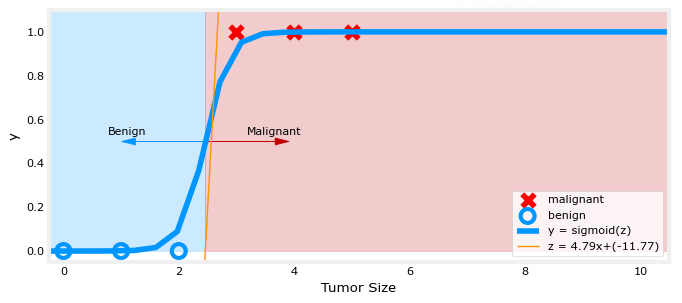
\includegraphics[width=\columnwidth]{logis-eg2}
			\caption{Example graph of logistic regression.\cite{enwiki:1188449633}}
			\label{fig:logis-eg2}
		\end{figure}
		
		\subsubsection{Decision Boundary}
		In a binary classification problem, a \textit{decision boundary} is a hypersurface that partitions the underlying vector space into two sets, one for each class. The classifier will classify all the points on one side of the decision boundary as belonging to one class and all those on the other side as belonging to the other class.\cite{enwiki:1152354295}

		In general, there are two types of decision boundary, linear decision boundary and nonlinear decision boundary.
		
		When $z$ is a linear function then logistic regression using $f_{\mathbf{w},e}(\mathbf{x})=g(z)$ learns to find a linear decision boundary like the one shown in Figure \ref{fig:decision}.
		
		On the other hand, if $z$ is a non-linear function, then just for example we let $z=w_1x_1+w_2x_2+w_3x_1^2+w_4x_2^2+e$ and logistic regression using $f_{\mathbf{w},e}(\mathbf{x})=g(z)$ learns to find a nonlinear decision boundary like the one shown in Figure \ref{fig:decision}.
		\begin{figure}[H]
			\centering
			\makebox[\columnwidth][c]{
				\subfloat[Linear decision boundary]{\scalebox{0.5}{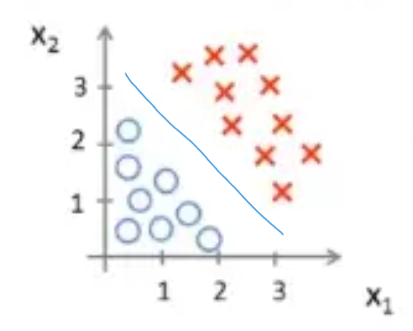
\includegraphics[width=\columnwidth]{linear-decision-boundary}}\label{fig:linear-decision}}
				\quad
				\subfloat[Nonlinear decision boundary]{\scalebox{0.5}{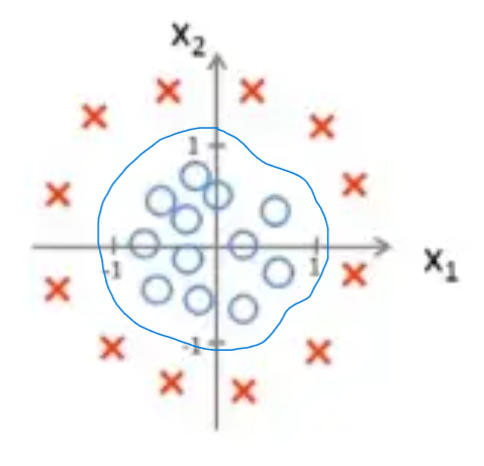
\includegraphics[width=\columnwidth]{non-linear-decision-boundary}}\label{fig:nonlinear-decision}}
			}
			\caption{Examples of decision boundary}
			\label{fig:decision}
		\end{figure}
		
		\subsubsection{New Cost Function}
		In linear regression, the cost function we use is squared error cost function. What if we stick with that convention? As shown in Figure \ref{fig:cost-nonconvex}, the curve is no longer convex which means by gradient descent we cannot reach its global minimum. Therefore a new cost function is needed.
		\begin{figure}[H]
			\centering
			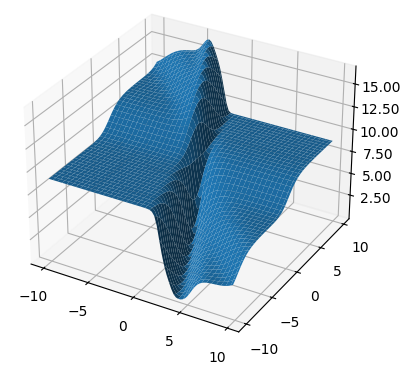
\includegraphics[width=\columnwidth]{squared-cost-of-sigmoid}
			\caption{Squared error cost function when applied to logistic regression}
			\label{fig:cost-nonconvex}
		\end{figure}
		We define Loss Function $L(f_{\mathbf{w},e}(\mathbf{x}),y)$, such that
		$$ J_{\mathbf{w},e}(\mathbf{x})=\frac{1}{m}\sum_{i=1}^{m}L(f_{\mathbf{w},e}(\mathbf{x^{(i)}}),y^{(i)}) $$
		Now what we need to do is to modify the Loss Function. And Logistic Loss Function is of the form:
		\begin{align*}
			&L(f_{\mathbf{w},e}(\mathbf{x^{(i)}}),y^{(i)}) \\
			&= \begin{cases}
				-\ln(f_{\mathbf{w},e}(\mathbf{x^{(i)}})) &\text{if }y^{(i)} = 1 \\
				-\ln(1 - f_{\mathbf{w},e}(\mathbf{x^{(i)}})) &\text{if }y^{(i)} = 0
			\end{cases} \\
			&= \begin{aligned}[t]
				&-y^{(i)}\ln(f_{\mathbf{w},e}(\mathbf{x^{(i)}})) \\
				&-(1-y^{(i)})\ln(1 - f_{\mathbf{w},e}(\mathbf{x^{(i)}}))
			\end{aligned}
		\end{align*}
		
		\subsubsection{Formula for Gradient Descent}
		The big formula for gradient descent is:
		\begin{align*}
			&\text{Repeat until convergence \{}\\
			&\qquad w_i\coloneq w_i-\alpha\frac{\partial J(\mathbf{w},e)}{\partial w_i} \\
			&\qquad\qquad\qquad\text{for }i=1,2,\cdots,n \\
			&\qquad e\coloneq e-\alpha\frac{\partial J(w,e)}{\partial e} \\
			&\text{\}}
		\end{align*}
		
		Now with change of $J(\mathbf{w},e)$, we need to re-calculate the partial derivative term\cite{derivative-of-logis}.
		
		\paragraph{Step 1} Derivative of the sigmoid function:
		$$
		\begin{aligned}[t]
			& g(x)=\frac{1}{1+e^{-x}} \\
			& \mathbf{\frac{d(g(x))}{dx}}
			\begin{aligned}[t]
				&= \frac{e^{-x}}{(1+e^{-x})^2} \\
				&= \frac{1}{1+e^{-x}}-\frac{1}{(1+e^{-x})^2} \\
				&= \frac{1}{1+e^{-x}}(1-\frac{1}{1+e^{-x}}) \\
				&= \mathbf{g(x)(1-g(x))}
			\end{aligned}
		\end{aligned}
		$$
		
		\paragraph{Step 2} Derivative of the cost function:
		$$
			J_{\mathbf{w},e}(\mathbf{x})
			\begin{aligned}[t]
			 	&=\frac{1}{m}\sum_{i=1}^{m}L(f_{\mathbf{w},e}(\mathbf{x^{(i)}}),y^{(i)}) \\
				&=\begin{aligned}[t]
					&\frac{1}{m}\sum_{i=1}^{m}\big(-y^{(i)}\ln(f_{\mathbf{w},e}(\mathbf{x^{(i)}})) \\
					&-(1-y^{(i)})\ln(1 - f_{\mathbf{w},e}(\mathbf{x^{(i)}}))\big)
				\end{aligned}
			\end{aligned}\\
		$$
		$$
			\frac{\partial J_{\mathbf{w},e}(\mathbf{x})}{\partial w_j}
			\begin{aligned}[t]
				&=\begin{aligned}[t]
					&\frac{1}{m}\sum_{i=1}^{m}\bigg(-y^{(i)}\frac{\partial\ln(f_{\mathbf{w},e}(\mathbf{x^{(i)}}))}{\partial w_j} \\
					&-(1-y^{(i)})\frac{\partial\ln(1 - f_{\mathbf{w},e}(\mathbf{x^{(i)}}))}{\partial w_j}\bigg)
				\end{aligned}\\
				&=\begin{aligned}[t]
					&\frac{1}{m}\sum_{i=1}^{m}\bigg(
					-y^{(i)}\frac{1}{f_{\mathbf{w},e}(\mathbf{x^{(i)}})}\\
					&\frac{\partial f_{\mathbf{w},e}(\mathbf{x^{(i)}})}{\partial w_j}-(1-y^{(i)})\\
					&\frac{-1}{1 - f_{\mathbf{w},e}(\mathbf{x^{(i)}})}
					\frac{\partial f_{\mathbf{w},e}(\mathbf{x^{(i)}})}{\partial w_j}\bigg)
				\end{aligned}\\
				&=\begin{aligned}[t]
					&\frac{1}{m}\sum_{i=1}^{m}
					\frac{\partial f_{\mathbf{w},e}(\mathbf{x^{(i)}})}{\partial w_j}\bigg(
					\frac{-y^{(i)}}{f_{\mathbf{w},e}(\mathbf{x^{(i)}})}\\
					&+\frac{1-y^{(i)}}{1 - f_{\mathbf{w},e}(\mathbf{x^{(i)}})}\bigg)
				\end{aligned}\\
				&=\begin{aligned}[t]
					&\frac{1}{m}\sum_{i=1}^{m}
					\frac{\partial f_{\mathbf{w},e}(\mathbf{x^{(i)}})}{\partial w_j}\\
					&\frac{f_{\mathbf{w},e}(\mathbf{x^{(i)}})-y^{(i)}}{f_{\mathbf{w},e}(\mathbf{x^{(i)}})(1 - f_{\mathbf{w},e}(\mathbf{x^{(i)}}))}\\
				\end{aligned}\\
				&=\frac{1}{m}\sum_{i=1}^{m}\big(
					f_{\mathbf{w},e}(\mathbf{x^{(i)}})-y^{(i)}
					\big)w_j
			\end{aligned}
		$$
		This little practice of calculus leads to a coincidence that the updating rules of both linear regression and logistic regression end up into a identical form.
		
	\subsection{Bias and Variance}
	When it comes to deploying an ML system, it is barely possible that your system makes perfect inference without further refinement and ML practitioners always endeavor to find equilibrium between bias and variance.
	\begin{figure}[H]
		\centering
		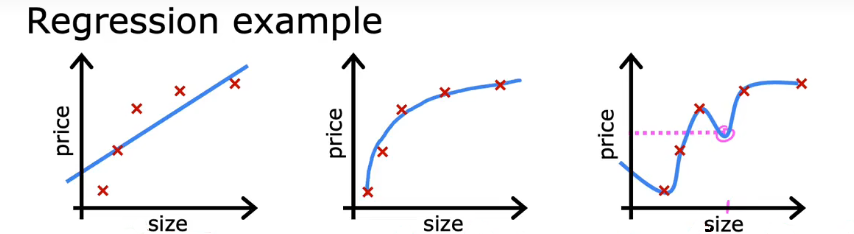
\includegraphics[width=\columnwidth]{bias-variance-eg}
		\caption{Scenarios where there is high bias or high variance.}
		\label{fig:bias-variance}
	\end{figure}
		\subsubsection{High Bias}
		Also known as Underfitting, high bias is a scenario where a model is unable to capture the relationship between the input and output variables accurately, generating a high error rate on both the training set and unseen data. It occurs when a model is too simple, which can be a result of a model needing more training time, more input features, or less regularization. 
		
		\subsubsection{High Variance}
		Overfitting is a concept in data science, which occurs when a model fits exactly against its training data. When this happens, the algorithm unfortunately cannot perform accurately against unseen data, defeating its purpose. Generalization of a model to new data is ultimately what allows us to use machine learning algorithms every day to make predictions and classify data.
		
		\subsubsection{Regularization}
		Particularly in ML, \textit{Regularization} is a process that changes the result answer to be 'simpler'\cite{regularization}. It is often used to prevent overfitting. Intuitively, penalty should be given to large parameters $w$ and to fulfill this a regularization term is added to the cost function:
		$$ J_{\mathbf{w},e}(\mathbf{x})=\frac{1}{m}\sum_{i=1}^{m}L(f_{\mathbf{w},e}(\mathbf{x^{(i)}}),y^{(i)})+\frac{\lambda}{2m}\sum_{j=1}^{n}w_j^2 $$
		
		Therefore, the formula for gradient descent is rewritten as:
		$$ \frac{\partial J_{\mathbf{w},e}(\mathbf{x})}{\partial w_j}=
		\begin{aligned}[t]
			&\frac{1}{m}\sum_{i=1}^{m}\big(f_{\mathbf{w},e}(\mathbf{x^{(i)}})-y^{(i)}\big)w_j \\
			&+\frac{\lambda}{m}w_j
		\end{aligned} $$
		
		\paragraph{Regularized Linear Regression}
		It is a common scenario in which a high order polynomial regression is overfitting a dataset. In Figure \ref{fig:regularization}, the green and blue functions both incur zero loss on the given data points. A learned model can be induced to prefer the green function, which may generalize better to more points drawn from the underlying unknown distribution, by adjusting $\lambda$, the weight of the regularization term.
		
		\paragraph{Regularized Logistic Regression}
		Same dilemma also applies to logistic regression. A high order polynomial may drive logistic regression model to fit a wiggly decision boundary as shown in Figure \ref{fig:regularization}. To make our model more generalizable, we apply regularization to tell the model to fit a more intuitively feasible decision boundary.

		\begin{figure}[H]
			\centering
			\makebox[\columnwidth][c]{
				\subfloat[Example of regularized linear regression.]{\scalebox{0.5}{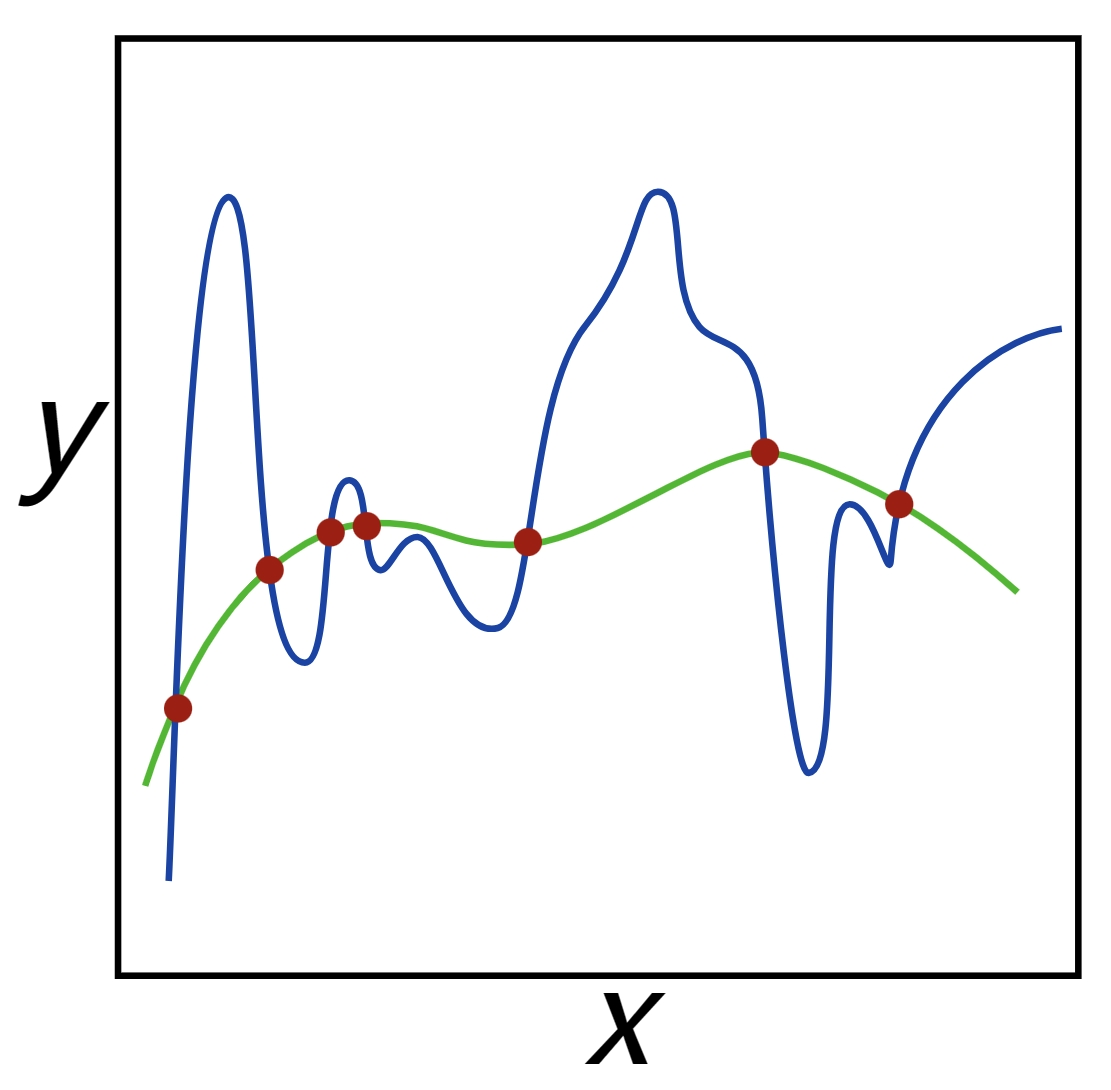
\includegraphics[width=\columnwidth]{linear-regularization-eg}}\label{fig:linear-regulation}}
				\quad
				\subfloat[Example of regularized logistic regression.]{\scalebox{0.5}{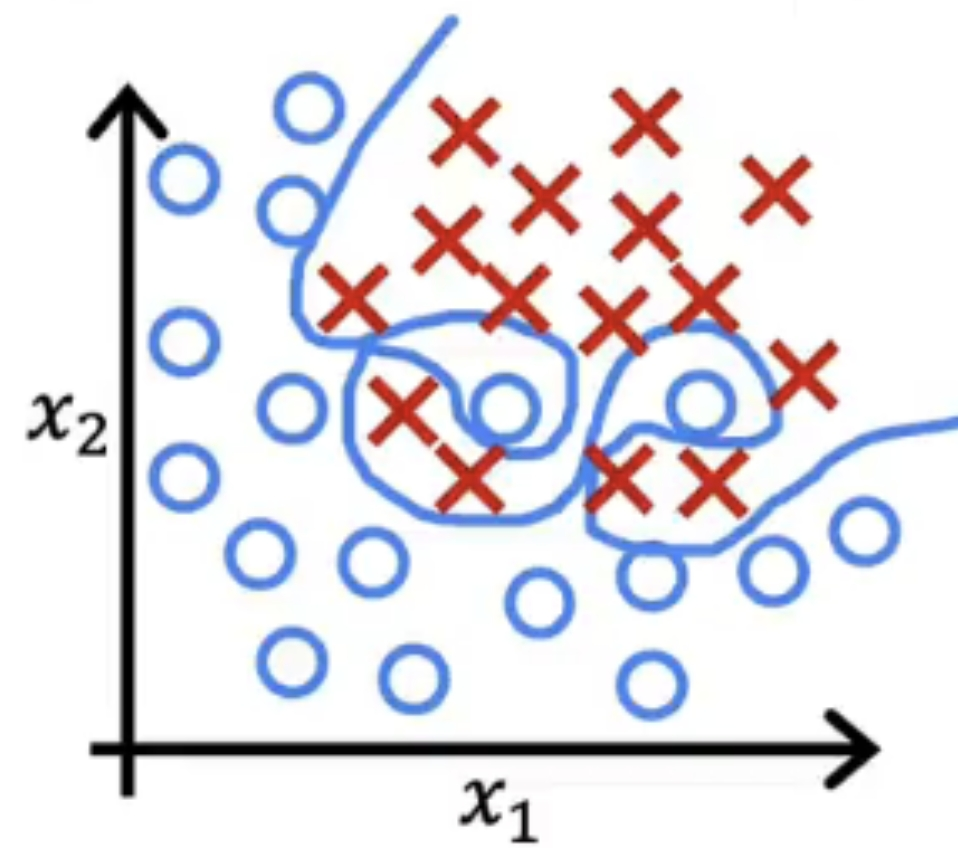
\includegraphics[width=\columnwidth]{logis-regularization-eg}}\label{fig:logis-regulation}}
			}
			\caption{Examples of decision boundary}
			\label{fig:regularization}
		\end{figure}
		
\section{Wrap-up}
In conclusion, while machine learning (ML) has undeniably revolutionized various fields, it is crucial to acknowledge and address its inherent limitations. One significant constraint lies in the dependency of ML models on vast amounts of labeled data for effective training. This requirement often proves challenging, especially in domains where obtaining labeled data is resource-intensive or impractical. Additionally, ML models may struggle with generalization when faced with unseen or outlier data, highlighting the importance of robustness and adaptability in future developments.

Furthermore, the interpretability of ML models remains a persistent challenge. Many advanced ML algorithms, particularly deep learning models, operate as "black boxes," making it difficult for users to comprehend the decision-making processes behind their predictions. This lack of transparency raises ethical concerns, particularly in sensitive applications such as healthcare and finance. Striking a balance between model complexity and interpretability will be crucial for fostering trust and facilitating widespread adoption of ML technologies.

Looking ahead, the future of artificial intelligence (AI) holds tremendous promise. Emerging technologies, such as reinforcement learning and unsupervised learning, are pushing the boundaries of what ML can achieve. These advancements offer the potential to overcome current limitations and pave the way for more sophisticated and versatile AI systems. Researchers and practitioners are encouraged to explore these cutting-edge algorithms, contributing to the ongoing evolution of AI and unlocking new possibilities across diverse industries.

The journey of machine learning is an ongoing expedition, marked by breakthroughs and challenges alike. As we navigate through the complexities of ML, it is essential to remain vigilant about its limitations and actively seek innovative solutions. Embracing a future perspective, one that involves the exploration of advanced AI algorithms, will not only enhance the capabilities of machine learning but also drive the continued advancement of artificial intelligence as a whole. As we stand on the cusp of a new era in technology, the collective efforts of researchers, developers, and enthusiasts will undoubtedly shape the trajectory of AI, opening doors to unprecedented opportunities and transformative possibilities.


\printbibliography
		
\end{multicols*}

\end{document}
